\documentclass[a4paper]{jpconf}
\usepackage{graphicx}
\usepackage{subfig}
\usepackage{booktabs}
\begin{document}
\title{Study of the high energy Cosmic Rays large scale anisotropies with the ANTARES neutrino telescope}

\author{G Illuminati}

\address{``La Sapienza'' University of Roma and INFN, Piazzale Aldo Moro, 5, 00185 Roma, Italy}


\ead{giulia.illuminati@roma1.infn.it}

\begin{abstract}
We present the analysis method used to search for an anisotropy in the high energy Cosmic Rays (CRs) arrival distribution using data collected by the ANTARES telescope. ANTARES is a neutrino detector, where the collected data are dominated by a large background of cosmic ray muons. Therefore, the background data are suitable for high-statistics studies of cosmic rays in the Northern sky. The main challenge for this analysis is accounting for those effects which can mimic an apparent anisotropy in the muon arrival direction: the detector exposure asymmetries, non-uniform time coverage, diurnal and seasonal variation of the atmospheric temperature. Once all these effects have been corrected, a study of the anisotropy profiles along the right ascension can be performed.
\end{abstract}

\section{Introduction}
Cosmic rays in the TeV to PeV range are mainly charged particles, believed to originate in our Galaxy, possibly in local astrophysical accelerators such as supernova remnants. After escaping from their sources, CRs propagate through the interstellar medium where they undergo a scattering process due to the presence of magnetic fields. Therefore, they are deflected from their original direction and their trajectories are efficiently isotropized before their arrival at Earth. However, it is predicted that a dipolar anisotropy with an amplitude of $\sim 10^{-3}$ or lower should subsist in their arrival directions. Such a large-scale anisotropy was observed at TeV energies by detectors in the Northern hemisphere, e.g. Tibet AS$\gamma$ \cite{tibet}, Super-Kamiokande-I \cite{superk} and Milagro \cite{milagro}, and then, in the Southern hemisphere, by IceCube \cite{ice}. The measured deviation from an isotropic distribution is of the order of 0.1$\%$ and the excess region and deficit region have the size of several tens degrees. 


\section{The ANTARES neutrino telescope}
The ANTARES neutrino telescope \cite{ageron}, located in the Northern hemisphere, at a depth of 2475 m in the Mediterranean Sea, about 40 km off the French coast near Toulon, is the first undersea neutrino telescope. Its main purpose is to detect high energy neutrinos from galactic and extragalactic sources \cite{point}. Neutrinos are detected indirectly through the detection of Cherenkov light produced by the path in water of relativistic muons emerging from charged-current muon neutrino interactions in the surroundings of the detector. ANTARES consists of an array of 12 lines anchored to the sea bed and maintained vertical by buoys, connected to a junction box which distributes the electrical power and transmits the data to shore through an  electro-cable. Each line supports 25 storeys made of triplets of 10-inch photomultipliers (PMTs) orientated  at  45$^{\circ}$ downwards  in  order  to  maximize  the sensitivity to Cherenkov light from up-going muons. The PMTs are used to detect the Cherenkov photons which produce a signal whose charge and time information are exploited to recostruct the direction of the muon.

\section{Data selection} 
The data used for this analysis were collected during the period January 2009 to December 2011 with a 12-line detector configuration. The recostruction strategy of the events is based on a maximum likelihood method in which the best set of parameters describing the track is estimated through a recursive fit procedure used to maximise the likelihood function. This function is the pdf of time residuals defined as the difference between theoretical and measured arrival times of the hits on the PMTs.  

The following cuts have been applied in order to keep only events that are \emph{suitable} for the analysis. The cut on the zenith angle, $\theta < 78^{\circ}$, ensures that only down-going
events are kept. Only events reconstructed with more than one line have been used since the cylindrical simmetry of the line prevents from obtaining a good reconstruction of the azimuth angle for the single-line events. The cut on the reconstructed energy, $E > 1$TeV, retains events in the energy range in which the anisotropy has been observed.


\section{Data - Montecarlo comparison}
The Montecarlo (MC) sample of events used in this analysis is performed with the MUPAGE \cite{mupage} package which simulates the propagation of the muons produced after the interaction of cosmic rays in the atmosphere. It is a run-by-run simulation: using the measured optical background rates, optical modules conditions and run duration, a realistic simulation of the physics and data taking process for each run is obtained. The comparison between data and simulations is an important step for this analysis: a good agreement between data and MC constitutes a necessary condition to investigate the presence of a possible anisotropy in the arrival distribution of data events compared to those isotropically simulated. Therefore, the first aim of the analysis is to identify the necessary cuts which provide a good agreement between data and MC distributions. The following cuts on the recononstruction quality parameter, $\Lambda$, and on the estimated angular error, $\beta$, have been applied: $\Lambda > -6.2$ and $\beta < 1^{\circ}$. Morever, those events whose track, at the moment of minimum approach to the axis of the detector, is still too far (distance from the detector center on the orizontal plane grater than 50 m and along the vertical axis grater than 200 m) have been rejected. Even if the described cuts have improved the agreement, the simulations are not precise at a level better than a few percent which is not at the required level  for anisotropies with amplitudes in the $10^{-4} - 10^{-3}$ range. Therefore,  in the analysis method used in this work, the MC distributions are not used to correct real data but the two samples are treated separately and then compared at the end of the analysis.  

\section{Corrections for spatial asymmetries}
An effect which must be accounted for in this analysis is an asymmetry in the ANTARES detector response due to the geometrical configuration of the lines (as shown in figure \ref {fig:azi} (a)) which results in a variable muon detection efficiency, as a function of the muon direction, as according to the azimuth angle, the number of strings encountered by the muon varies. To correct this effect, each event in a certain week $j$ from a given local azimuth bin $i$ was weighted with the ratio $\frac{\bar{n}}{n_i}$ where $\bar{n}$ is the average number of events over the full range of local azimuths in the week $j$, and $n_i$ is the number of events in local azimuth bin $i$.
This method allows to obtain weights that take into account the fact that the detector is subjected to enviromental conditions which vary over short periods. 
Figure \ref {fig:azi} (b) shows an example of the azimuth distribution for the week 24/12/2011 - 31/12/2011 with the horizontal red line denoting $\bar{n}$ for that week.


\begin{figure}[!h]
\centering
\subfloat[][]
{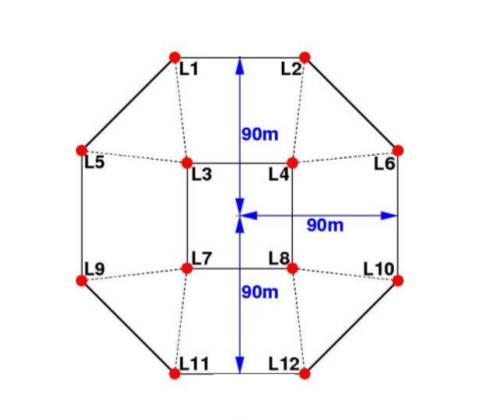
\includegraphics[width=.40\columnwidth]{Fig_1}} \quad
\subfloat[][]
{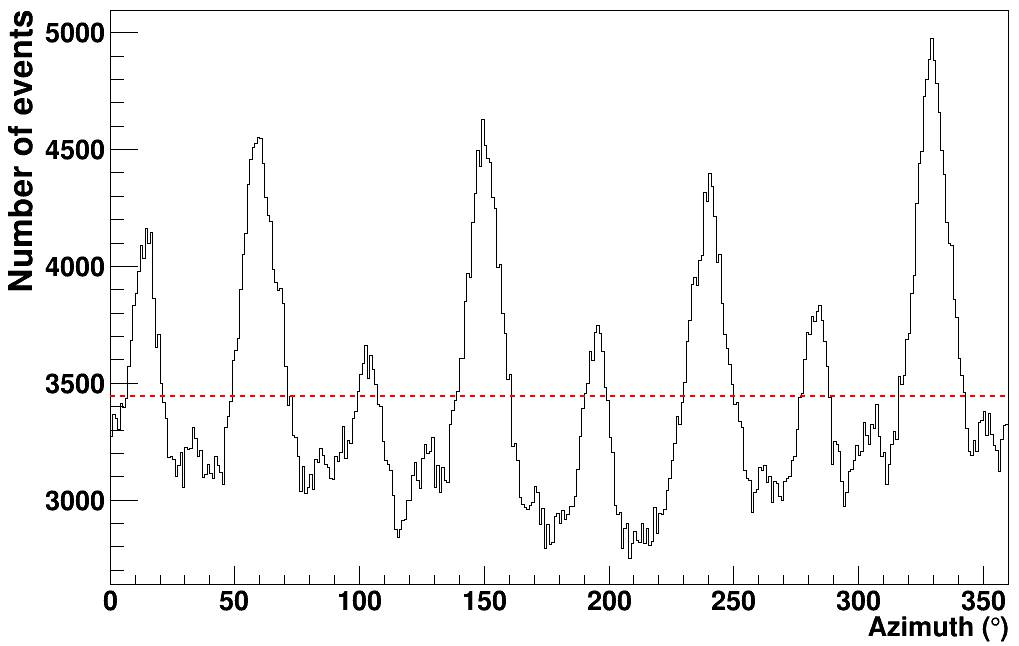
\includegraphics[width=.40\columnwidth]{Fig_2}}
\caption{(a) Lines arrangement in the detector. (b) Azimuth distribution for the period 24/12/2011 - 31/12/2011. The dashed red line shows the value of $\bar{n}$ for the distribution.    }
\label{fig:azi}
\end{figure}

In addition to the azimuthal asymmetry a non-uniform $cos\theta$ distribution is observed. Figure \ref {fig:cz2} shows the $cos\theta$ and zenith distributions for the whole sample after the described corrections.
\begin{figure}[!h]
\centering
\subfloat[][]
{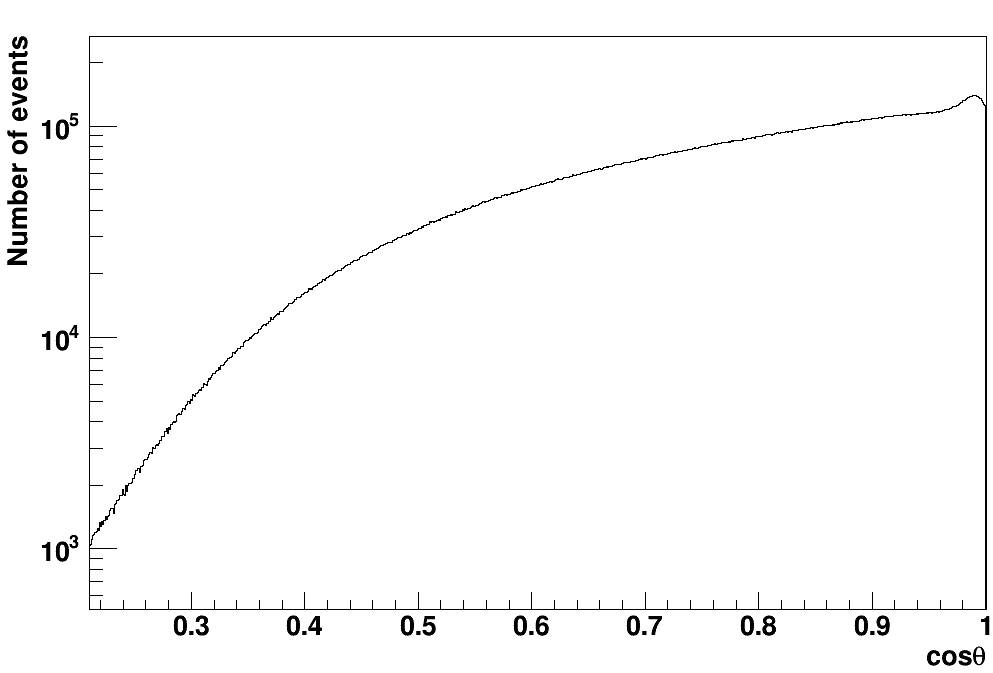
\includegraphics[width=.40\columnwidth]{Fig_3}} \quad
\subfloat[][]
{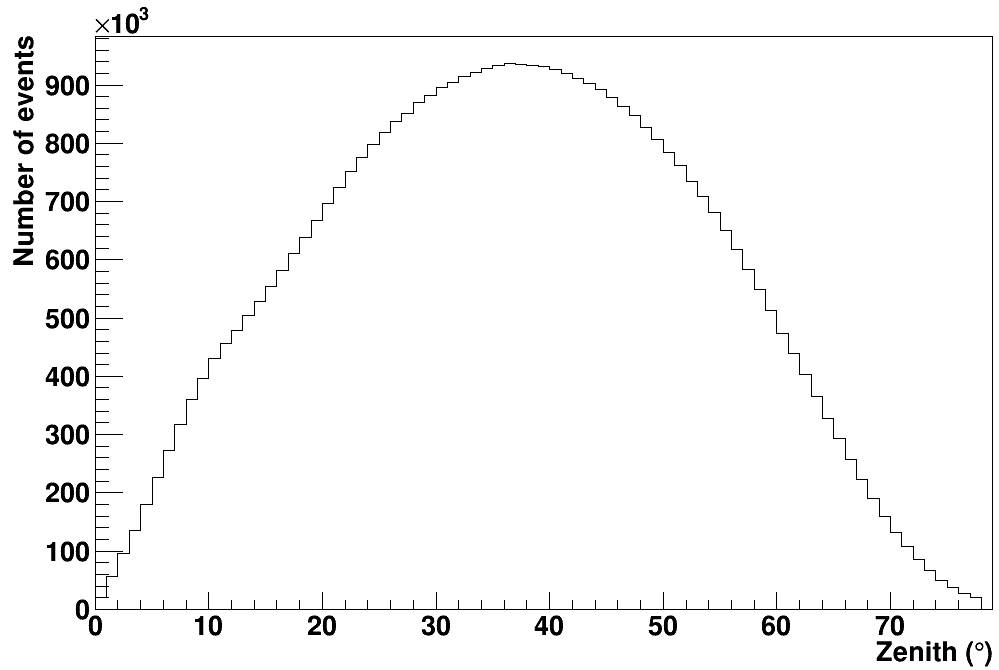
\includegraphics[width=.40\columnwidth]{Fig_4}}
\caption{$Cos\theta$ (a) and Zenith (b) distribution for the period 01/01/2009 - 31/12/2011 after the corrections for the detector geometrical asymmetry have been applied.}
\label{fig:cz2}
\end{figure}
It is evident that more events arrive from $ 20^{\circ}\le \theta \le 50^{\circ}$ compared to those arriving from the zenith and the horizon. This is in contrast with the uniform distribution in cos$\theta$ that is expected at the entrance of the atmosphere if the flux of CRs is isotropic and it is due to several effects and selection criteria applied to the secondary muons events. 
Since it is known that the primary CRs distribution in the upper atmosphere is uniform in $cos\theta$, the idea is to exploit the distribution of secondary muons as an estimate of the overall ANTARES efficiency in detecting CRs by means of downgoing atmospheric muons. Such efficiency can be found normalising the $cos\theta$ distribution to its maximum value.
The correction for this effect is then obtained by weighting each real and MC event from a given local $cos\theta$ bin $i$ by the relative efficiency $w_i = \frac{1}{eff(cos\theta _i)}$.


\section{Corrections for non-uniform temporal exposure}
Another effect which must be accounted for is the non-uniformity in the time coverage of the data: gaps in the detector uptime and uneven run selection due to quality selection
introduce non-uniformities into the time coverage of the data which translate into an artificial arrival direction asymmetry in equatorial coordinates. 
In order to estimate the ``exposure'' map in equatorial coordinates (right ascension $\alpha$ and declination $\delta$), the following procedure has been used. 
The duration of each run $k$ in the analysed period has been divided in minutes and, for each minute, every couple of coordinates ($\phi_m$,$\theta_n$), in the visible range ($ 0^{\circ} \le \phi < 360^{\circ}$ and $0^{\circ} \le \theta \le 78^{\circ}$), has been converted in the corresponding couple of equatorial coordinates ($\alpha _i$,$\delta _j$) that has then been used to fill a 2-dim histogram $E^k_{i,j}=E^k(\alpha _i , \delta _j)$, with a $6^{\circ} \times 6^{\circ}$ binning.
The sum over the total amount of runs $N$ of the exposition in each angular bin $\sum_{k=1}^{N} E^k_{i,j}$ gives the coverage map for every couple $(\alpha _i , \delta _j)$. Normalising the obtained map to its maximum value provides a new set of weights, functions of the equatorial coordinates, defined as the fraction of the total live time of the detector during the three years in which each angular bin has been visible. 

\section{Corrections for atmospheric temperature}
Another possible effect that can modify the observed muon flux, causing an apparent anisotropy, is the seasonal variation of the atmospheric temperature. Indeed, increases of the air temperature during summer lower the average gas density; the less dense medium allows a longer mean free path of the mesons and increases the fraction of them that decay to produce muons before their first interaction. Since the atmospheric temperature varies over seasonal periods, it is expected to observe a seasonal modulation in the muon flux as well. Such correlation has already been largely observed and studied by experiments like Macro \cite{art:macro}, MINOS \cite {art:minos} and Borexino \cite {art:borexino}. 

Since meson decays take place over a range of altitudes where the temperature is changing, it is customary to define an effective atmospheric temperature $T$, obtained from a weighted average over atmospheric depth \cite{grashorn}. The variation in the observed muon rate $R_{\mu}$ compared to the mean rate over the total data-taking period $<{R}_{\mu}>$  can be  expressed in terms of a similar change in $T$ as:

{
\small
\begin{equation}
\centering
\label{eq:temp}
\frac{R_{\mu}-<R_{\mu}>}{<R_{\mu}>} = \alpha _T \frac{T-<T>}{<T>}
\end{equation}
}

where $\alpha_T$ is the ``effective temperature coefficient'' whose magnitude depends upon the muon energy and hence upon the depth of the detector ($\alpha _T$ is about 0.95 for the ANTARES depth). In this analysis, we have raplaced the muon rate with the ratio between real and simulated events, $R = N_{data} /N_{MC}$, since $R$ shows smaller fluctuations than $R_{\mu}$. This substitution is valid since possible correlations with the atmospheric temperature are not taken into account in the simulation of MC events. 
Figure \ref {label} shows the obtained trend of $\Delta R/ <R>$ versus $\Delta T/ <T>$, both averaged over periods of 15 days, and the theoretical linear trend. 

\begin{figure}[h]
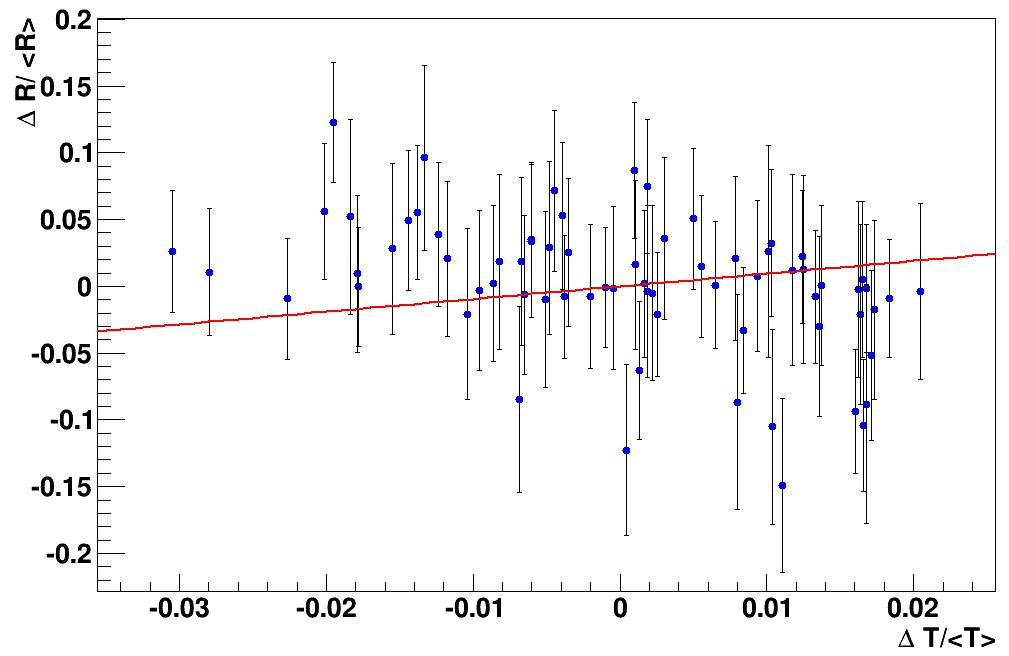
\includegraphics[width=20pc]{Fig_5}\hspace{2pc}%
\begin{minipage}[b]{14pc}\caption{\label{label}$\Delta R/ <R>$ versus $\Delta T/ <T>$ for the analysed period. The solid red line shows the theoretical linear trend.}
\end{minipage}
\end{figure}

Temperature fluctuations of the order of $\pm 3\%$ can be observed which lead to an expected $R$ fluctuation of $\sim 2.85\%$ according to eq. \ref {eq:temp}. However, figure \ref {label} shows statistical fluctuations of the ratio between data and MC of the order of $10\%$. Even if the used data sample with the applied cuts, due to high statistical uncertainties, does not show a correlation with the atmospheric temperature, such correlation is a well known effect already observed by several experiments. Therefore, we have decided to apply the correction due to the atmospheric temperature to the number of observed muons. In particular, each event in a certain 15 days period $p$ has been multiplied by a weight estimated from the averaged temperature in the same period according to eq. \ref {eq:temp}:

\begin{equation}
\centering
\label{eq:pesot}
w_p=\frac{1}{\alpha _T (\frac{\Delta T}{<T>})_p +1}
\end{equation}

\section{Analysis of the anisotropy}
The corrections described in the previous sections have been adopted in order to obtain the map in equatorial coordinates of the number of observed events as a function of their true arrival direction, so that a possible large scale anisotropy can be verified. In order to study the anisotropy along the right ascension (R.A.), we divide the map in equatorial coordinates in 30$\times$60 angular bins ($\Delta \delta = 6^{\circ}$, $\Delta \alpha = 6^{\circ}$). For each $6^{\circ}$ declination band we evaluate the weighted average of the number of events $\bar{n}_{\delta _j} = \frac{1}{\sum P_{i,j}} \sum_{i=1}^{60} n(\alpha _i , \delta _j)P_{i,j}$. This value is used to normalize to 1 the content of each bin in R.A., $n(\alpha _i, \delta _j)$, providing the relative intensity map in which anisotropies are expressed as deviations from 1. Then, the anisotropy profile is obtained as the 1D projection in the R.A. direction of the 2D relative intensity map. Figure \ref {fig:fit} shows the anisotropy profiles along the R.A. for data (a) and MC (b). Both trends have been fitted with the equation of a horizontal line and with a first harmonic function in order to test the hypothesis of uniform and dipolar trend.  Figure \ref {fig:fit} also shows the result of the fits.  The parameters values obtained with the fit are reported in table \ref {ex}. 

\begin{figure}[h!]
\centering
\subfloat[][]
{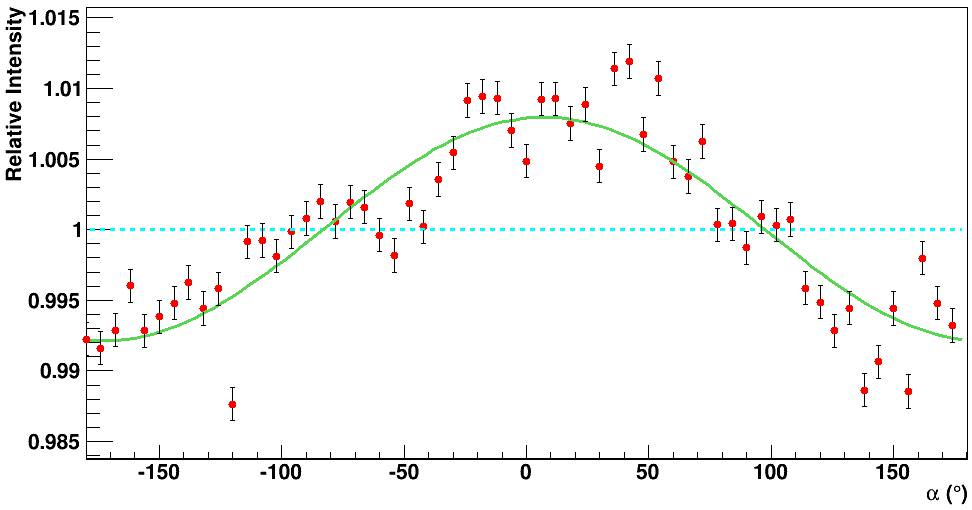
\includegraphics[width=.48\columnwidth]{Fig_6}} \quad
\subfloat[][]
{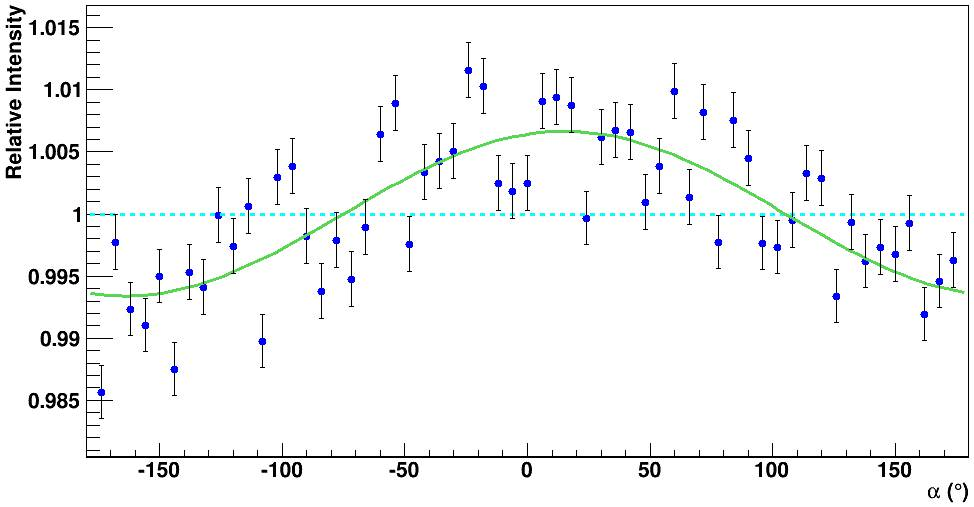
\includegraphics[width=.48\columnwidth]{Fig_7}}
\caption{Anisotropy profiles for data (a) and MC (b). The results of the fit are also shown: the dashed light blue line shows the linear fit ($y = m x + q$ with $m=0$), the solid green line shows the fit with the first harmonic ($y= A_1 cos(x - \phi _1) + B$).}
\label{fig:fit}
\end{figure}

\begin{table}[h]\footnotesize
\caption{\label{ex} Columns 1, 2: result from the linear fit $y = m x + q$ with $m=0$ .  Columns 3, 4, 5, 6: result from the fit with the first harmonic $y= A_1 cos(x - \phi _1) + B$. }
\begin{center}
\lineup
\begin{tabular}{llllllll}
\br
& $q$ & $\chi ^{2}/ndf$& $A_1 (10^{-3}) $ & $\phi _1 (^{\circ})$ & $B$ & $\chi ^{2} /ndf$\\ 
\mr
\textbf{data} & $1.0000 \pm 0.0001$ & $1678/59$& $7.92 \pm 0.22$ & $0.12 \pm 0.03$ & $1.0000 \pm 0.0001$ & $333/57$ \\
\textbf{MC} & $1.0000 \pm 0.0002$ & $476/59$& $6.62 \pm 0.40$ & $0.26 \pm 0.06$ & $1.0000 \pm 0.0003$ &$198/57$\\
\br
\end{tabular}
\end{center}
\end{table}

Since the distributions show a large dispersion of data, it is unlikely to find a function which represents satisfactorily the obtained trends. The parameters obtained from the fit suggest that for both data and MC the hypothesis of constant value is the worst description of the distributions.
Concerning the fit with the harmonic, it is evident that the hypothesis of oscillatory trend cannot be totally excluded for the MC events, whose distributions are expected to be uniform after corrections. This implies that there could still be, in the analysis procedure for example, a systematic effect that causes an apparent anisotropy.   
However, the fit with the harmonic gives different values of amplitudes and phases for the data distribution with respect to the MC. This suggests that the modulation effect along the R.A. in the MC distribution is not coincident with the one which causes the modulation in the data distribution.

\section{Conclusions}
In this work, data collected by the ANTARES detector in the period 01/01/2009 - 31/12/2011 have been analysed with the intention of searching for the large scale anisotropy in the high energy primary Cosmic Rays arrival directions. Since several factors can mimic an apparent anisotropy preventing from obtaining the real distributions of data, the main challenge was to remove such systematic effects with a series of corrections. Then, in order to quantify the scale of the anisotropy in the obtained corrected maps, the right ascension dependence of the data has been fitted to a first order harmonic function together with a line, used to test the hypothesis of uniform trend for the MC distribution. The obtained results with the harmonic fit suggests that the modulation effect along the R.A. in the distribution cannot be explained by the same effect which causes the modulation in the MC distribution. The observed ``modulation'' in R.A., that could reflect a higher muon rate in particular seasons of the year, could be related to residual effects due to bioluminescence: higher background could increase the number of ``fake'' muons but also enlarge the efficiency in real track reconstruction. A larger data sample could give us the possibility to harden the selection cuts and then to remove any residual systematic effects. 

%%%%%%%%%%%%%%%%%%%%%%%%%%%%%%%%%%%%%%%%%%%


\section*{References}
\begin{thebibliography}{9}
\bibitem{tibet} Amenomori M \emph{et al} 2006 \emph{Science} \textbf{314} 439
\bibitem{superk} Guillain G \emph{et al} 2007 \emph{Phys. Rev.} D \textbf{75} 062003
\bibitem{milagro} Abdo A  \emph{et al} 2009 \emph{Astrophys. J.} \textbf{698} 2121
\bibitem{ice} Abbasi R \emph{et al} 2010 \emph{Astrophys. J.} \textbf{718} L 194 
\bibitem{ageron}  Ageron M \emph{et al}  2011 \emph{Nucl. Instrum. Meth. } A \textbf{656} 11
\bibitem{point} Adrian-Martinez S \emph{et al} 2014 \emph{Astrophys. J. Lett.} \textbf{786} L5
\bibitem{mupage} Carminati G, Bazzotti M, Margiotta A and Spurio M 2008 \emph{Compututer Physics Communications} \textbf{179} 915
\bibitem{art:macro} Ambrosio M \emph{et al} 1997 \emph{Astropart. Phys.} \textbf{7} 109.
\bibitem{art:minos} Adamson P \emph{et al} 2010 \emph{Phys. Rev.} D\textbf{81} 012001
\bibitem{art:borexino} Bellini G \emph{ et al} 2012 \emph{ J. Cosm. Astropart. Phys.} 1205  015 
\bibitem{grashorn} Grashorn E \emph{et al} 2010 \emph{Astropart. Phys.} \textbf{33} 140.

\end{thebibliography}

\end{document}


